%____________________WEEK 3_____________________________%
\newpage
\section{Tuần 3}
\subsection{Bài toán cần giải quyết}
\begin{itemize}
    \item \textbf{Bài toán:} Nhận diện các chữ số viết tay.
    \item \textbf{Sơ lược về mô hình:} \cite{model} Mô hình nhận đầu vào (input) là hình ảnh có kích thước \textbf{28x28 pixel} chứa một chữ số bất kỳ từ \textbf{0 đến 9}, sau đó dự đoán và đưa ra kết quả là một số nguyên tương ứng với chữ số xuất hiện trong hình ảnh nhận được ban đầu.
\end{itemize}

\subsection{Dữ liệu và phân chia dữ liệu}
- Dữ liệu được sử dụng trong mô hình này là tập dữ liệu \textbf{MNIST} \cite{mnist} được lấy từ website kaggle.com bao gồm 4 file:
\begin{figure}[H]
    \centering
    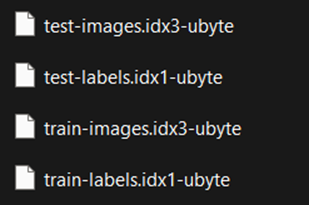
\includegraphics[width=0.5\linewidth]{img/dataset.png}
    \caption{Các tập dữ liệu}
\end{figure}
\begin{itemize}
    \item Trong đó:
    \begin{itemize}
    \item File \texttt{test-images.idx3-ubyte} chứa 60.000 hình ảnh có kích thước 28x28 pixel là các chữ số viết tay của tập huấn luyện (train set).
    \item File \texttt{train-labels.idx1-ubyte} chứa các nhãn là các chữ số tương ứng với từng hình ảnh của tập huấn luyện.
    \item File \texttt{test-images.idx3-ubyte} chứa 10.000 hình ảnh có kích thước 28x28 pixel là các chữ số viết tay của tập kiểm tra (test set).
    \item File \texttt{test-labels.idx1-ubyte} chứa các nhãn là các chữ số tương ứng với từng hình ảnh của tập kiểm tra.
\end{itemize}
\end{itemize}

- Các hình ảnh trong tập dữ liệu đều có nền là màu đen và nét màu trắng thể hiện một chữ số bất kỳ từ 0 đến 9.\\
\begin{figure}
    \centering
    
\includegraphics[width=0.4\linewidth]{img/data_sample.png}
    \caption{Ví dụ một hình ảnh của tập dữ liệu thể hiện chữ số 3}
\end{figure}

- Tiếp theo, sử dụng phương thức \texttt{train\_test\_split} từ thư viện \texttt{scikit-learn} lên train set để tạo ra được một tập dữ liệu mới là validation set. Lúc này, train set sẽ được tách ra thành hai tập ngẫu nhiên với 5\% là validation set và phần còn lại là train set.
\\- Vậy ta sẽ có được ba tập dữ liệu sẽ được sử dụng cho các bước sau của mô hình:
\begin{itemize}
    \item \textbf{Train set}:  Sử dụng để huấn luyện và tinh chỉnh các tham số của mô hình.
    \item \textbf{Validation set}: Sử dụng để kiểm tra độ chính xác của mô hình trong quá trình học xem mô hình có thích nghi tốt với tập dữ liệu chưa từng thấy bao giờ hay không, từ đó có thể giảm thiểu vấn đề overfitting.

    \item \textbf{Test set}: Sử dụng để kiểm tra độ hiệu quả của mô hình sau khi được huấn luyện.
\end{itemize}

\subsection{Thiết kế, huấn luyện mạng neutral}

\subsubsection{Kiến trúc neural network}
\begin{enumerate}
    \item \textbf{Xây dựng mô hình neural network:}
    \begin{itemize}
        \item Kiến trúc: Mô hình neural network được sử dụng là một multilayer perceptron gồm một lớp đầu vào (input layer), một lớp ẩn (hidden layer) và một lớp đầu ra (output layer). 
        \begin{itemize}
            \item Input layer: Gồm 784 nút, mỗi nút thể hiện một pixel trên ma trận ảnh 28x28
            \item Hidden layer(s): Mô hình này sẽ chỉ gồm 1 lớp ẩn duy nhất gồm 10 nút. Dữ liệu từ lớp Input sẽ thông qua hàm Linear và hàm ReLu để tính toán kết quả đầu ra cho lớp ẩn. 
            \item Output Layer: Gồm 10 nút thể hiện các chữ số từ 0 đến 9. Kết quả đầu ra từ lớp ẩn sẽ thông qua hàm Linear để có được kết quả đầu ra cho lớp Output. Giá trị của mỗi nút là xác suất mà hình ảnh ban đầu chứa chữ số tương ứng mà nút đó thể hiện. Kết quả dự đoán của mô hình là nút có xác suất cao nhất. 
        \end{itemize}
        \item Trong quá trình huấn luyện: kết quả từ lớp Output sẽ thông qua hàm mất mát (trong mô hình này là Cross-Entropy) kết hợp với hàm softmax để tính toán sai số giữa đầu ra dự đoán của mô hình và đầu ra thực tế.
        \item Sau khi đi qua tất cả các lớp và tính toán được sai số của mô hình. Ta sẽ cập nhật các tham số (Weight và Bias) bằng thuật toán lan truyền ngược (back propagation) và Stochastic Gradient Descen (SGD) optimizer.
    \end{itemize}
    \item \textbf{Khởi tạo các tham số của neural network:}
    \begin{itemize}
        \item \texttt{Imput\_dim = 784}: Kích thước của lớp input
        \item  \texttt{Hidden\_dim = [10]}: Một danh sách gồm các kích thước của từng lớp ẩn
        \item \texttt{Output\_dim = 10}: Kích thước của lớp output 
        \item \texttt{Regularization}: Hằng số được thêm vào quá trình tính gradient để giảm hiện tượng overfitting 
        \item \texttt{Learning Rate}: Tốc độ học của mô hình ($lr$) 
    \end{itemize}
    \item \textbf{Xây dựng các class cơ bản:}
    \begin{itemize} 
        \item \texttt{Linear}: là một hàm tuyến tính được biểu diễn qua phương trình
        \begin{center}
        \large $y = w \times x + b$
        \end{center}
        Trong đó: 
        \begin{itemize}
            \item $y$: kết quả đầu ra của hàm linear 
            \item $w$: trọng số (Weight)
            \item $x$: giá trị đầu vào của hàm 
            \item $b$: hệ số bias  
        \end{itemize}
        \item \texttt{ReLu}: Nếu không có các hàm kích hoạt phi tuyến, thì mạng neural của chúng ta dù có nhiều lớp vẫn sẽ có hiệu quả như một lớp tuyến tính. Vì vậy cần có sự xuất hiện của một hàm phi tuyến trong mô hình. Trong mô hình này, ta sẽ sử dụng hàm ReLu. Hàm ReLu được định nghĩa như sau: 
        \begin{center}
        \large $R(x) = max(0,x)$
        \end{center}
        Trong đó 
        \begin{itemize}
            \item $x$: giá trị đầu vào của hàm. 
        \end{itemize}
    \end{itemize}
    
    
\end{enumerate}
\subsubsection{Quá trình huấn luyện mô hình}
- Mô hình được huấn luyện thông qua 2 quá trình: \textbf{lan truyền tiến} (Forward propagation) và \textbf{lan truyền ngược} (Back propagation)
\begin{enumerate}
    \item \textbf{Lan truyền tiến:}
    \\- Trong quá trình lan truyền tiến, giá trị đầu vào từ lớp \texttt{Input} là ma trận \texttt{X} sẽ được sử dụng để tính toán giá trị của lớp \texttt{Hidden} là \texttt{$H_1$}, sau đó giá trị \texttt{$H_1$} sẽ tiếp tục được sử dụng làm giá trị đầu vào để tính toán giá trị của lớp \texttt{Output} là \texttt{scores}. Cuối cùng, ta sẽ sử dụng hàm một hàm mất mát là hàm \texttt{Cross-Entropy} để tính toán sai số \texttt{cost} giữa đầu ra dự đoán của mô hình là \texttt{scores} và đầu ra thực tế là \texttt{y}.
    \begin{figure}[H]
        \centering
        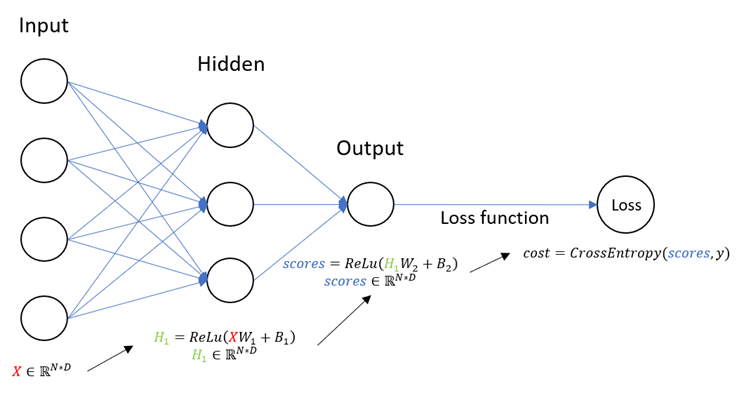
\includegraphics[width=0.7\linewidth]{img/Forward.png}
        \caption{Mô hình mô phỏng lan truyền tiến}
        
    \end{figure}
    \item \textbf{Lan truyền ngược:}
    \\- Sau khi tính toán được sai số giữa đầu ra dự đoán của mô hình và đầu ra thực tế, ta sẽ sử dụng sai số này để \textbf{điều chỉnh các tham số của từng lớp} sao cho giá trị đầu ra dự đoán gần với đầu ra thực tế nhất bằng cách lan truyền ngược. 
    \\- Các bước lan truyền ngược: Đầu tiên, ta \textbf{tính toán giá trị đạo hàm} của hàm mất mát đối với giá trị đầu ra dự đoán của mô hình. Sau đó ta sử dụng giá trị này kết hợp với quy tắc dây chuyền (chain rule) để tính toán đạo hàm của lớp \texttt{Output} rồi tiếp tục lấy đạo hàm của lớp \texttt{Output} để tính toán đạo hàm của lớp trước nữa. Nói cách khác, đạo hàm của lớp sau sẽ được lan truyền lại để tính đạo hàm của lớp trước thông qua quy tắc dây chuyền (chain rule).
    \begin{figure}[H]
        \centering
        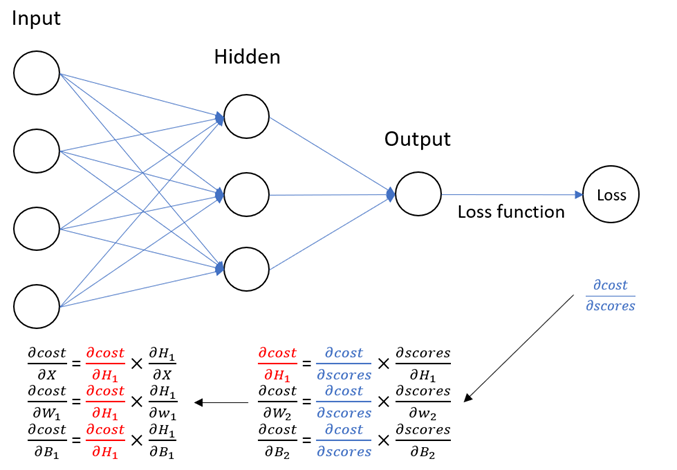
\includegraphics[width=0.7\linewidth]{img/backpropagation.png}
        \caption{Mô hình mô phỏng lan truyền ngược}
    \end{figure}
    - Sau khi tính toán được đạo hàm của từng tham số (Weight và Bias) trong từng lớp, ta sẽ sử dụng phương pháp gradient descent để \textbf{cập nhật lại các tham số} này nhằm giảm giá trị của cost.
    \begin{figure}[H]
        \centering
        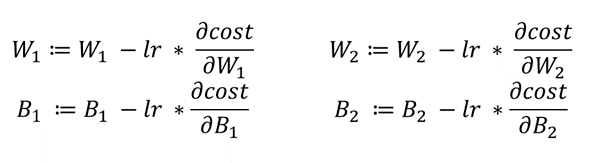
\includegraphics[width=0.75\linewidth]{gd_bias_weight.png}
        \caption{Công thức cập nhật tham số (Weight và Bias) của từng lớp}
        
    \end{figure}
\end{enumerate}


\subsubsection{Loss function: Cross-Entropy (CE) và hàm Softmax}
- \textbf{Cross-Entropy Loss function:} Là một loss function thường được sử dụng trong các bài toán phân loại bao gồm cả các mô hình neural network hoặc bài toán dự đoán xác suất. Hàm này đo lường mức độ sai lệch giữa hai phân phối xác suất: phân phối dự đoán của mô hình và phân phối thực tế. Công thức chung của Cross-Entropy Loss function cho hai phân phối xác suất P và Q là: 
    \begin{center}
        \large $CE = - \sum_{i=1}^{C} P_{i}\times \log(Q_{i})$
    \end{center}
    Trong đó:
    \begin{itemize}
        \item $C$: số lượng các class cần phân lớp.
        \item $Q_{i}$: xác suất thực tế của lớp thứ i
        \item $P_{i}$: xác suất dự đoán của lớp thứ i bởi mô hình
    \end{itemize}
- Đối với mô hình này, kết quả đầu ra của lớp Output có thể là các giá trị âm. Do đó, ta không thể trực tiếp sử dụng các giá trị này để tính toán sai số thông qua hàm Cross-Entropy được. Thay vào đó ta sẽ \textbf{chuẩn hóa các giá trị này bằng hàm Softmax} có hai tính chất là các xác suất luôn nằm trong khoảng (0, 1] và tổng các xác suất bằng 1. Sau đó sử dụng các giá trị đã chuẩn hóa này để tính toán sai số thông qua hàm Cross-Entropy. 
\\- Giả sử có một vector đầu vào $z = (z_1, z_2, ..., z_k)$, hàm Softmax sẽ tính xác suất $p_i$ cho mỗi phần tử theo công thức:
\begin{center}
    \Large $p_{i}=\frac{e^{z_{i}}}{\sum_{j=1}^{k}e^{z_{j}}},\forall i=1,2,...,k$
\end{center}

\subsubsection{Optimizer: Stochastic Gradient Descent (SGD)}
Stochastic Gradient Descent là một biến thể của Gradient Descent. Thay vì sau mỗi epoch chúng ta sẽ cập nhật trọng số một lần, thì trong mỗi epoch có N điểm dữ liệu, chúng ta sẽ cập nhật trọng số N lần. Nhờ sử dụng SGD nên tốc độ hội tụ của mô hình khá nhanh.
\begin{figure}[H]
    \centering
    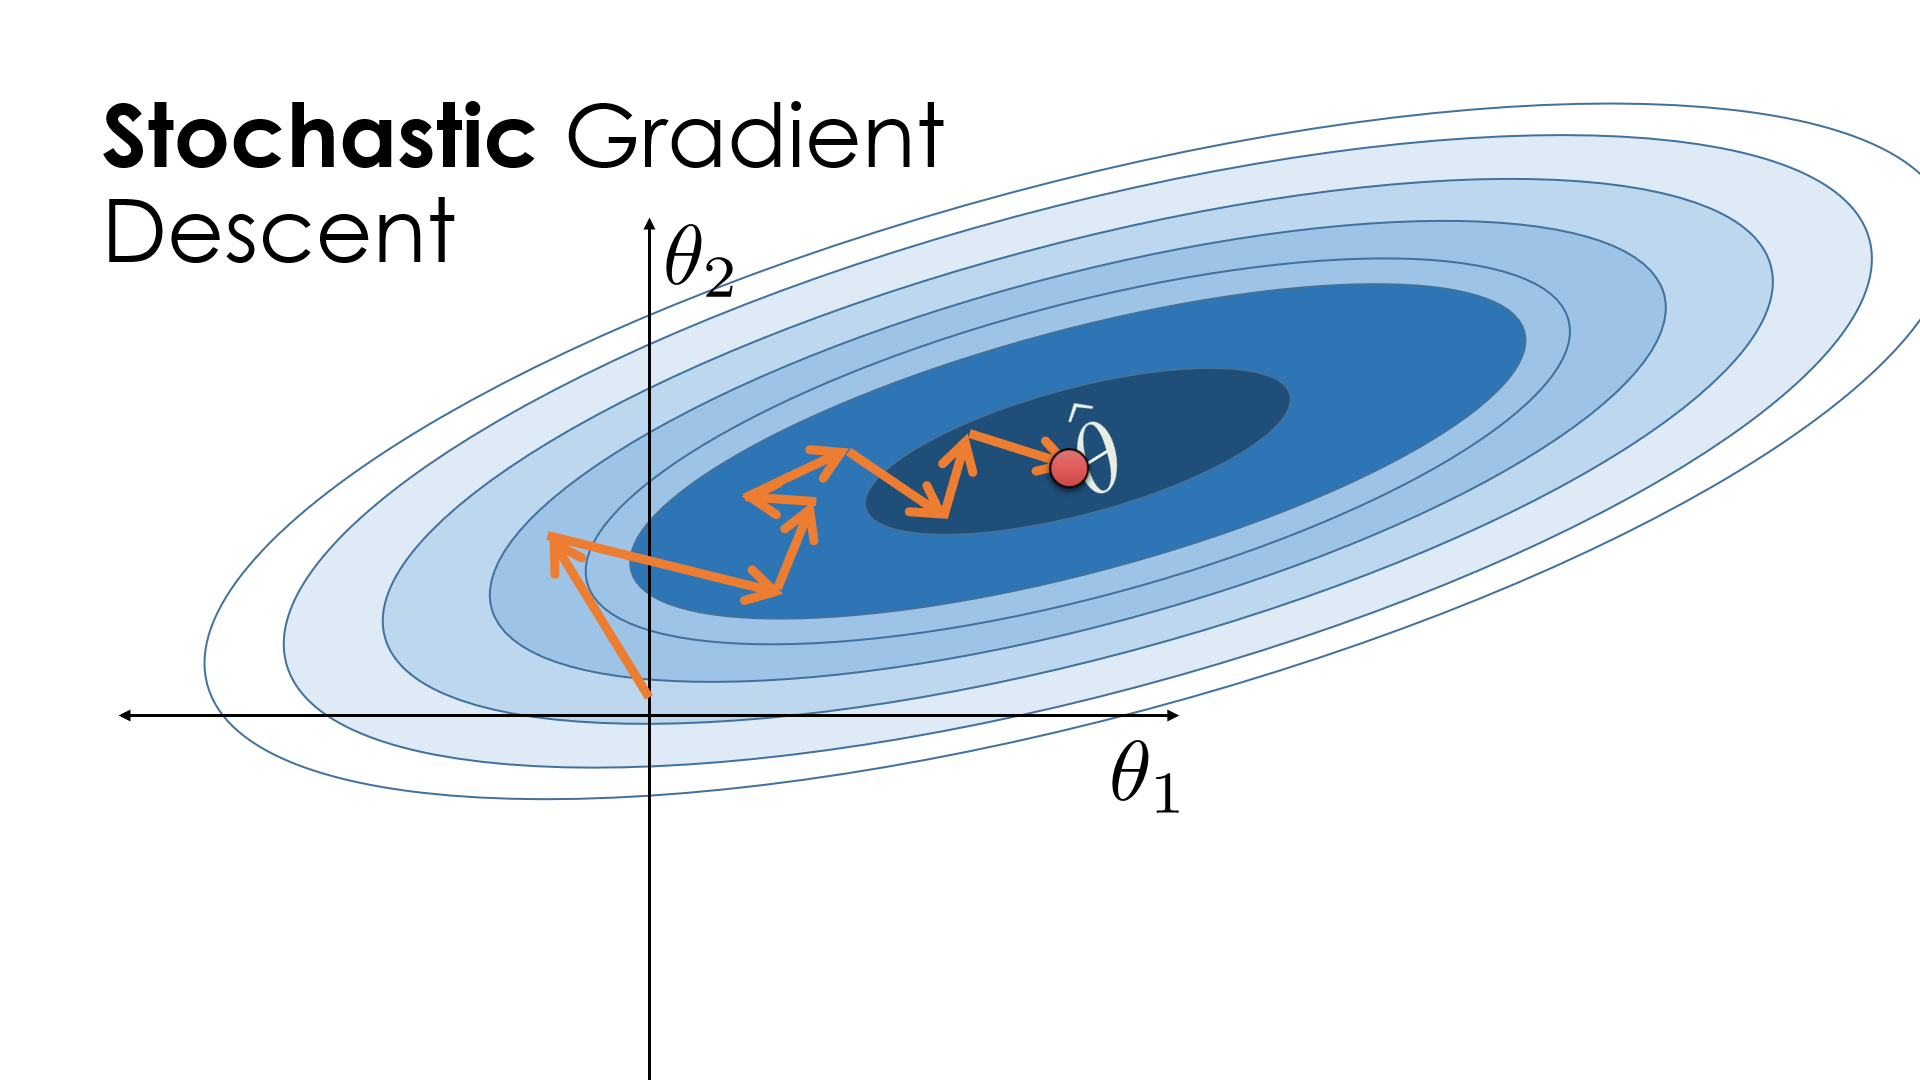
\includegraphics[width=0.75\linewidth]{img/SGD.png}
    \caption{Stochastic Gradient Descent}
    
\end{figure}
\subsubsection{Learning rate, số epoch, batch-size, regularization}
- Learning rate, số epoch, batch-size và regularization là các thông số quan trọng trong việc quyết định tốc độ học và độ chính xác của mô hình.
\begin{enumerate}
    \item \textbf{Learning rate:} 
    \\- Ban đầu khởi tạo giá trị \texttt{learning\_rate} thủ công, cứ sau mỗi \texttt{decay\_after} lần lặp thì ta sẽ cập nhật giá trị \texttt{learning\_rate} mới bằng cách nhân với một lượng \texttt{learning\_rate\_decay} (với \texttt{learning\_rate\_decay} < 1). 
    \\- Điều này sẽ giúp tăng dần tính chính xác với \texttt{learning\_rate} giảm dần khi tiến lại gần điểm hội tụ, tránh trường hợp \texttt{learning\_rate} quá lớn dẫn đến việc phân kì. 
    \\- Các giá trị liên quan đến \textbf{learning rate} được khởi tạo như sau:
    \begin{itemize}
        \item $learning\_rate = 0.001$
        \item $decay\_after = 50$
        \item $learning\_rate\_decay = 0.99$
    \end{itemize}
    \item \textbf{Số epoch:} Số lần truyền tập train để huấn luyện cho neural network
    \begin{itemize}
        \item $epoch = 200$
    \end{itemize}
    \item \textbf{Batch-size:} Tách bộ dữ liệu train thành các batch nhỏ hơn với kích thước là \texttt{batch-size} để tối ưu tốc độ huấn luyện.
    \begin{itemize}
        \item $batch-size = 200$
    \end{itemize}
    \item \textbf{Regularization:} Hằng số được thêm vào quá trình tính gradient để giảm hiện tượng
overfitting 
    \begin{itemize}
        \item $Regularization = 5\times 10^{-6}$
    \end{itemize}
\end{enumerate}
\subsection{Quá trình hội tụ, kết quả kiểm thử mô hình}
\subsubsection{Quá trình hội tụ}
- Để tiện quan sát các giá trị cost sau mỗi epoch của tập train set và validation set, cứ sau mỗi 10 epoch thì ta hiển thị giá trị trung bình của hàm loss (average cost), độ chính xác của mô hình với tập train (train accuracy) và độ tương thích của mô hình đối với các tập dữ liệu mới (val accuracy).
\\- Giá trị cứ sau mỗi 10 epoch khi train mô hình ghi lại được: 
\begin{itemize}
    \item Epoch 10 – Train cost: 1.65, Validation Cost: 1.74 
    \item Epoch 20 – Train cost:1.16, Validation Cost: 1.33 
    \item Epoch 30 – Train cost: 0.9, Validation Cost: 1.03 
    \item Epoch 40 – Train cost: 0.75, Validation Cost: 0.89 
\end{itemize}
- Qua đó ta có thể thấy được: 
\begin{itemize}
    \item Train cost và Validation cost giảm dần theo sự tăng dần của epoch. 
    \item Đạt được mục tiêu của việc huấn luyện mô hình: giảm thiểu các giá trị của hàm loss, tăng độ chính xác của mô hình. 
    \item Huấn luyện dựa trên quá trình lan truyền tiến và ngược trong neural network giúp mô hình học được các mối quan hệ giữa input và output để cho ra dự đoán chính xác với những bộ dữ liệu mới ngoài tập train set. 
\end{itemize}
\begin{figure}[H]
    \centering
    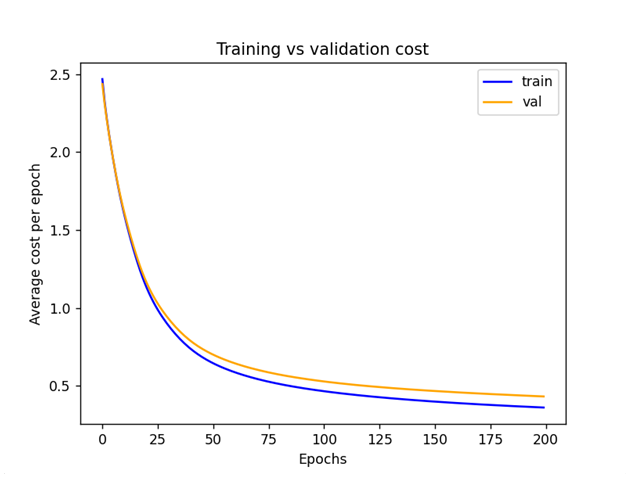
\includegraphics[width=0.75\linewidth]{img/hoitu.png}
    \caption{So sánh Training và Validation Cost}
\end{figure}
- Dựa vào biểu đồ minh họa sự thay đổi của 2 giá trị Train cost và Validation cost trên cả tập train set và validation set sau mỗi epoch, ta có nhận xét: 
\begin{itemize}
    \item Nếu cả hai cost giảm dần, cuối cùng hội tụ ổn định thì quá trình train của mô hình học tốt. 
    \item Nếu cost trên tập train set giảm dần trong khi cost trên tập validation tăng lên, có thể đây là dấu hiệu của overfitting. 
\end{itemize}

\subsubsection{Kết quả kiểm thử} 
\begin{itemize}
    \item Trong quá trình huấn luyện, giá trị của hàm loss (average cost) giảm dần và độ chính xác của train set và validation set tăng dần theo số lần lặp (epoch).
    \item Trong quá trình huấn luyện, ở \textbf{epoch cuối}:
    \begin{itemize}
        \item Giá trị cost trung bình: 0.36
        \item Độ chính xác (accuracy) trên train set: 89\%
        \item Độ chính xác (accuracy) trên validation set: 89\%
    \end{itemize}
    \item \textbf{Trong quá trình kiểm thử mô hình, độ chính xác (accuracy) trên test set: 89\%}
    \begin{figure}[H]
        \centering
        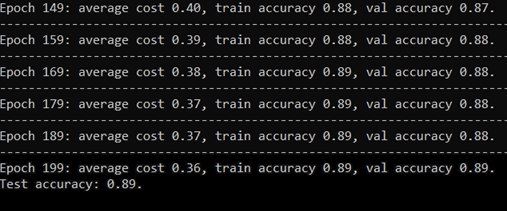
\includegraphics[width=0.75\linewidth]{img/testacc.png}
        \caption{Accuracy trên test set}
        
    \end{figure}
\end{itemize}

\subsection{Demo}

\begin{itemize}
    \item Link demo \cite{demo}: \href{https://www.youtube.com/watch?v=UQExhzgt-6E}{https://www.youtube.com/watch?v=UQExhzgt-6E} 
    \newpage
    \item 4 hình ảnh trong test set mà mô hình dự đoán đúng
    \begin{figure}[H]
    \centering
    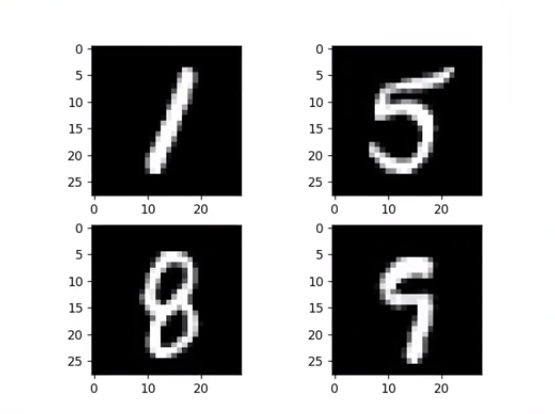
\includegraphics[width=0.65\linewidth]{true.png}
    \caption{Các mẫu mô hình dự đoán đúng}
        
    \end{figure}
    \item 4 hình ảnh trong test set mà mô hình dự đoán sai
    \begin{figure}[H]
    \centering
    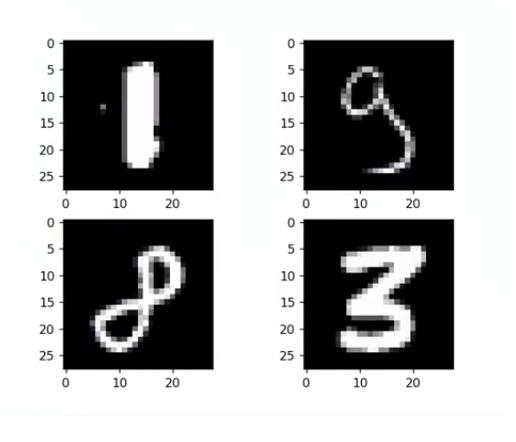
\includegraphics[width=0.65\linewidth]{img/false.png}
    \caption{Các mẫu mô hình dự đoán sai}
\end{figure}
\end{itemize}

